%% chapters/01-random-variables.tex
%% Chapter 1: Random Variables, A Working Vocabulary
%%
%% Section status:
%%   §1.0  Chapter opener + whereWeAre   DONE  (audit pass v0.4)
%%   §1.1  Sample spaces, outcomes, X    DONE  (audit pass v0.4 — anchors, cartoons, hints)
%%   §1.2  Distributions: PMF / PDF / CDF  placeholder
%%   §1.3  Expectation and variance        placeholder
%%   §1.4  Independence and joint distributions  placeholder
%%   §1.5  Brief warm-ups + chapter recap  placeholder

\chapter{Random Variables: A Working Vocabulary}
\label{ch:rvs}

\whereWeAre{%
This is the first chapter of the book. Everything that follows, moment generating functions, the central limit theorem, sample covariance matrices, eigenvalue fluctuations, and ultimately spectral clustering, is built on top of the language we develop here.\\[0.3em]
By the end of this chapter the reader will be able to: define random variables and their distributions cleanly, compute expectations and variances of all the running examples (Bernoulli, Binomial, Normal, Exponential), and recognize when two random variables are independent. The chapter assumes only basic high-school algebra and a willingness to draw a few pictures.%
}

% --- Page 11 chapter-opener cartoon -----------------------------------------
% AI-IMAGE SLOT: figures/ch01/wizard-comic.png
% Until that file exists, the TikZ fallback (\wizardHatCartoon) renders.
%
% PROMPT FOR THE IMAGE GENERATOR
% ------------------------------
% A 4-panel hand-drawn comic strip in the style of Calvin and Hobbes (Bill
% Watterson) or Sandra Boynton, soft pastel colors, warm friendly characters.
%
%   Panel 1: A young wizard character with a tall pointed hat (lilac purple,
%            roughly #8273A8) holds up a coin, looking curious. Speech
%            bubble: "Heads or tails?"
%
%   Panel 2: The wizard tosses the coin high in the air. The coin spins
%            mid-air with motion lines. The wizard looks up, expectant.
%
%   Panel 3: The coin lands on a table, balanced perfectly on its edge.
%            The wizard's eyes go wide in surprise.
%
%   Panel 4: The wizard scribbles on a chalkboard the equation
%            "P(edge) ~ 0", with a small sweat drop. Speech bubble:
%            "Probability is rigorous magic."
%
% Style: hand-drawn lines, soft pastel fills, warm off-white background
% (#F8F6F2), charcoal-gray ink lines (#2D2D2D), slight texture.  Use
% lilac, mustard, coral, mint, and soft gold accents.  No text outside
% speech bubbles.  Friendly, gently humorous, NOT slick or stylized like
% anime; closer to a children's book illustration that adults would also
% find charming.
%
% Aspect: ~3:4 portrait or 2x2 grid.  Rendered at margin width (~10pc).
% ----------------------------------------------------------------------
\marginnote{%
\centering
\anchorDot{1}\,\sffamily\footnotesize\scshape Mathemagics\par
\smallskip
\artOrTikz{figures/ch01/wizard-comic.png}{\wizardHatCartoon}\par
\smallskip
\itshape\footnotesize Probability is rigorous magic: we name the unknown, weigh it, and pull conclusions out of it.
}

Probability is the language\anchorDot{1} we use when we want to say something precise about a quantity that is uncertain. The outcome of a coin flip, the height of a randomly chosen person, the largest eigenvalue of a sample covariance matrix; all of these vary across repetitions of the experiment, and probability supplies the vocabulary for describing how. The unit of vocabulary is the \vocab{random variable}: a single number whose value is unknown until the experiment is run. This chapter builds that vocabulary from scratch and trains the running examples that the rest of the book will lean on.

\section{Sample spaces, outcomes, and the function we call \texorpdfstring{$X$}{X}}
\label{sec:rvs-samplespace}

Before we can define a random variable, we need to be precise about what it ``randomizes over.''\anchorDot{2} That requires three pieces:

\begin{enumerate}
\item an \vocab{experiment}, the act whose result is uncertain;
\item the \vocab{sample space} $\Omega$, the set of all possible outcomes of the experiment;
\item a \vocab{probability function} $\Prob$ that assigns a number in $[0,1]$ to events (i.e., subsets of $\Omega$), with $\Prob(\Omega) = 1$.
\end{enumerate}

% --- Page 12 margin: historical aside FIRST, then experiments ---------------
\asideHistorical{\anchorDot{2}\, The modern definition of a random variable as a function on a sample space is due to Andrey Kolmogorov, in his 1933 monograph \emph{Foundations of the Theory of Probability}. Before Kolmogorov, ``random'' was a word in search of a definition.}

\marginGap

\marginnote{%
\centering
\anchorDot{3}\,\sffamily\footnotesize\scshape Three running experiments\par
\medskip
{\renewcommand{\arraystretch}{2.2}%
\begin{tabular}{@{}c@{\quad}l@{}}
\coinbig{H}      & \footnotesize coin: $2$ outcomes\\
\diebig{3}       & \footnotesize die: $6$ outcomes\\
\tapeMeasureIcon & \footnotesize tape measure: a continuum
\end{tabular}}%
}

The simplest example is a single coin flip.\anchorDot{3} The experiment is the flip; the sample space is $\Omega = \{H, T\}$; and the probability function (for a fair coin) is $\Prob(H) = \Prob(T) = \tfrac{1}{2}$. The outcomes here are just the labels $H$ and $T$. They are not numbers, they are labels for possibilities.

Often we care less about the labels themselves than about a number we can compute from them. For two coin flips, we may care about the \emph{number of heads}; for the roll of two dice, we may care about the \emph{sum}; for a clinical trial, we may care about whether a patient recovered or not. In each case there is a function that takes an outcome and returns a number. That function is the random variable.\anchorDot{4}

\begin{definition}{Random variable}{rv}
\anchorDot{1}\,Let $\Omega$ be a sample space. A \emph{random variable} on $\Omega$ is a function $X : \Omega \to \R$ that assigns to each outcome $\omega \in \Omega$ a real number $X(\omega)$.\footnotemark
\end{definition}
\footnotetext{In a fully rigorous treatment we would also require $X$ to be \emph{measurable}; this technical condition becomes relevant only when $\Omega$ is uncountable. Appendix~D sketches the measure-theoretic framework for the curious reader.}

\asideMatters{\anchorDot{1}\, Defining $X$ as a function on $\Omega$, rather than just as ``a random number,'' lets us recover \emph{any} numerical question about the experiment by the same mechanism. The number of heads, the number of tails, whether the first flip matched the second; each is a different function on the same $\Omega$.}

\marginGap

\marginnote{%
\centering
\anchorDot{4}\,\sffamily\footnotesize\scshape A random variable as a machine\par
\smallskip
\begin{tikzpicture}[scale=0.55, every node/.style={font=\sffamily\footnotesize}]
  \node[anchor=east] at (-2.6, 0) {$\omega$};
  \draw[->, line width=0.55pt, mathemagicsThm] (-2.5, 0) -- (-1.05, 0);
  \draw[rounded corners=4pt, draw=mathemagicsThm, fill=mathemagicsIntuBg!70,
        line width=0.7pt]
    (-1, -0.85) rectangle (1, 0.85);
  \node[font=\itshape\bfseries\Large, color=mathemagicsDef] at (0, 0) {$X$};
  \draw[draw=mathemagicsThm, line width=0.4pt] (0, 0.95) circle (0.18);
  \foreach \angle in {0,45,90,135,180,225,270,315} {
    \draw[mathemagicsThm, line width=0.3pt]
      (0, 0.95) ++(\angle:0.18) -- ++(\angle:0.08);
  }
  \draw[->, line width=0.55pt, mathemagicsThm] (1.05, 0) -- (2.5, 0);
  \node[anchor=west] at (2.6, 0) {$X(\omega)$};
\end{tikzpicture}\par
\smallskip
\itshape\footnotesize Outcomes go in; numbers come out. The randomness lives in the input, not in the machine.
}

\begin{intuition}
Think of $X$ as a \emph{measurement device}. The randomness lives in $\Omega$; it is the underlying experiment whose outcome we cannot predict. The random variable $X$ does not introduce any new randomness; it just tells you what number you record once an outcome has been drawn.
\end{intuition}

To see what the definition means in practice, take the simplest non-trivial example.

% --- Page 13 margin: cartoon coin at the start of this subsection -----------
% AI-IMAGE SLOT: figures/ch01/coin-cartoon.png
% Until that file exists, the TikZ fallback (\coinCartoon) renders.
%
% PROMPT FOR THE IMAGE GENERATOR
% ------------------------------
% A hand-drawn cartoon coin character with personality, in the style of a
% Sandra Boynton illustration or a friendly children's book.
%
% The coin is a large round shape (cream / pale-yellow #FBF3D9 fill, with a
% charcoal #2D2D2D outline), shown front-on.  The coin has a face: two big
% round eyes (wide open with curiosity), small expressive eyebrows raised
% in question, and a small smile.  The letter "H" is prominently embossed
% on the coin's face below the eyes.
%
% The coin is mid-thought.  To the right, a small thought bubble (white,
% charcoal outline) trails up from the coin's head with two small puffs
% leading up to a larger speech-bubble shape.  Inside the bubble, in a
% friendly serif font, is the equation: "P(H) = 1/2".
%
% Style: warm hand-drawn ink, soft pastel palette, off-white background
% (#F8F6F2).  Charcoal lines, mustard / cream coin body, no harsh shading.
% Inviting, gently humorous.  The coin is being asked a question and is
% genuinely thinking about it.
%
% Aspect: square (1:1).  Rendered at margin width (~10pc).
% ----------------------------------------------------------------------
\marginnote{%
\centering
\anchorDot{5}\,\sffamily\footnotesize\scshape Heads or tails?\par
\smallskip
\artOrTikz{figures/ch01/coin-cartoon.png}{\coinCartoon}\par
\smallskip
\itshape\footnotesize One coin flip is the simplest non-trivial experiment in all of probability.
}

\begin{example}{Number of heads in two coin flips}{two-coin-flips}
\anchorDot{5}\,Flip a fair coin twice in a row. The sample space contains four outcomes,
\[
\Omega \;=\; \{HH,\; HT,\; TH,\; TT\},
\]
each with probability $\tfrac{1}{4}$. Define the random variable
\[
X(\omega) \;=\; \text{the number of heads in } \omega.
\]
Then $X(HH) = 2$, $X(HT) = 1$, $X(TH) = 1$, and $X(TT) = 0$. So $X$ takes its values in $\{0, 1, 2\} \subset \R$. \cref{fig:rv-mapping} draws the function: outcomes on the left, sorted by their image; the real number line on the right; arrows from each outcome to its target, with $HT$ and $TH$ visibly converging at $1$.
\end{example}

\begin{figure}[h]
\centering
\begin{tikzpicture}[
  >={Stealth[length=4.5pt]},
  every node/.style={font=\sffamily},
  outcome/.style={
    font=\footnotesize\sffamily, color=mathemagicsThm,
    inner sep=2pt
  },
  arr/.style={
    ->, thick, draw=mathemagicsIntu, line width=0.55pt,
    shorten >=2pt, shorten <=2pt
  },
  realline/.style={->, line width=0.6pt, draw=mathemagicsThm}
]
\node[font=\itshape\sffamily, color=mathemagicsThm, anchor=south]
     at (0, 2.25)
     {\large $X = $ ``number of heads in two coin flips''};

\fill[mathemagicsDefBg, rounded corners=8pt]
  (-3.5, -2.0) rectangle (-1.3, 2.0);
\node[font=\sffamily\itshape\bfseries, color=mathemagicsThm,
      anchor=north west]
     at (-3.4, 1.95) {$\Omega$};

\node[outcome] at (-2.4, 1.5)   (hh) {HH};
\node[outcome] at (-2.4, 0.35)  (ht) {HT};
\node[outcome] at (-2.4,-0.35)  (th) {TH};
\node[outcome] at (-2.4,-1.5)   (tt) {TT};

\draw[realline] (3, -1.95) -- (3, 1.95)
  node[above, font=\sffamily, color=mathemagicsThm] {$\R$};
\foreach \y/\lbl in {-1.5/0, 0/1, 1.5/2} {
  \draw[mathemagicsThm, line width=0.5pt] (2.85, \y) -- (3.15, \y);
  \node[right=4pt, font=\footnotesize\sffamily, color=mathemagicsThm]
       at (3.15, \y) {$\lbl$};
}

\draw[arr] (hh.east) -- (2.84, 1.5);
\draw[arr] (ht.east) -- (2.84, 0);
\draw[arr] (th.east) -- (2.84, 0);
\draw[arr] (tt.east) -- (2.84,-1.5);

\node[font=\itshape\sffamily, color=mathemagicsIntu, above=1pt]
     at (0.2, 1.5) {$X$};

\end{tikzpicture}
\caption[The random variable $X$ as a function from $\Omega$ to $\R$.]{The random variable $X$ assigns to every outcome $\omega \in \Omega$ a real number $X(\omega)$. Outcomes that share a value share a target on the line: here $HT$ and $TH$ both map to $1$, which is why $\Prob(X{=}1) = \tfrac{1}{2}$. Layout adapted from~\citep{nrich-rv}.}
\label{fig:rv-mapping}
\end{figure}

Before moving to a richer example, two notational conventions are worth pinning down. They will be used everywhere in this book.

\begin{definition}{Notation: $X$ versus $x$}{notation}
Capital letters ($X$, $Y$, $Z$, \ldots) denote random variables, the \emph{functions} on $\Omega$. Lowercase letters ($x$, $y$, $z$, \ldots) denote particular real numbers, specific values that those random variables \emph{could} take.
\end{definition}

So when we write $\Prob(X = x)$, we are asking: what is the probability that the random variable $X$ takes the value $x$? In the two-coin example above,
\[
\Prob(X = 0) = \tfrac{1}{4}, \qquad
\Prob(X = 1) = \tfrac{1}{2}, \qquad
\Prob(X = 2) = \tfrac{1}{4}.
\]
The probability $\Prob(X = 1) = \tfrac{1}{2}$ comes from the fact that two of the four equally-likely outcomes ($HT$ and $TH$) map to $1$.

A second example, with a richer sample space, exercises the same pattern.

\marginnote{%
\centering
\anchorDot{2}\,\sffamily\footnotesize\scshape One outcome, sum $= 7$\par
\smallskip
\diebig{3}\quad\diebig{4}\par
\smallskip
\itshape\footnotesize One of six pairs that sum to seven; the others are $(\die{1},\die{6})$, $(\die{2},\die{5})$, $(\die{4},\die{3})$, $(\die{5},\die{2})$, $(\die{6},\die{1})$.
}

\begin{example}{Sum of two dice}{two-dice}
Roll two fair six-sided dice.\anchorDot{2} The sample space contains $36$ ordered pairs:
\[
\Omega = \bigl\{(i, j) : i, j \in \{1, 2, 3, 4, 5, 6\}\bigr\},
\]
each with probability $\tfrac{1}{36}$. Let $X(i, j) = i + j$ be the sum. Then $X$ takes values in $\{2, 3, \ldots, 12\}$, and the probability of each value is the number of $(i, j)$ pairs that sum to it, divided by $36$:
\[
\Prob(X = 2) = \tfrac{1}{36}, \quad \Prob(X = 7) = \tfrac{6}{36}, \quad \Prob(X = 12) = \tfrac{1}{36}.
\]
The full distribution of $X$\anchorDot{3} has the familiar triangular shape: rare on the extremes (only one pair sums to $2$), most likely in the middle (six different pairs sum to $7$). \cref{fig:dice-distribution} plots it.
\end{example}

\begin{marginfigure}
\centering
\anchorDot{3}\par\smallskip
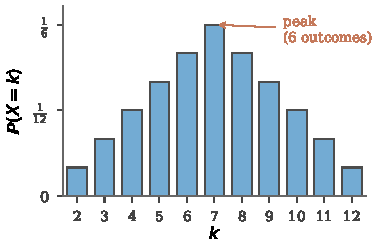
\includegraphics[width=\linewidth]{figures/ch01/dice-distribution.pdf}
\caption{The distribution of $X$ in \cref{ex:two-dice}. The triangular peak at $k = 7$ is no coincidence: of the $36$ equally-likely pairs $(i, j)$, exactly $6$ sum to $7$.}
\label{fig:dice-distribution}
\end{marginfigure}

This is the working pattern. We start from a sample space whose outcomes carry no numerical structure; we define a function $X$ that turns each outcome into a number; and we pull the probabilities forward through $X$ to talk about $\Prob(X = x)$ or, more generally, $\Prob(X \in A)$ for any subset $A$ of $\R$.
\newpage
\subsection*{Brief warm-ups}

\hint{\anchorDot{4}\,How many outcomes do you get from flipping three coins? Try listing them in order, then count those with exactly $k$ heads.}
\begin{warmup}[\coffee{1}]
Three coins are flipped, all fair, all independent.\anchorDot{4} Write down the sample space $\Omega$. Define the random variable $X$ to be the number of heads. List $X(\omega)$ for each $\omega \in \Omega$, and compute $\Prob(X = k)$ for $k = 0, 1, 2, 3$.
\end{warmup}
\begin{warmupSolution}
$\Omega = \{HHH, HHT, HTH, HTT, THH, THT, TTH, TTT\}$, eight outcomes each with probability $\tfrac{1}{8}$. The values of $X$ are $3, 2, 2, 1, 2, 1, 1, 0$ respectively. Counting,
$\Prob(X{=}0) = \tfrac{1}{8}$,
$\Prob(X{=}1) = \tfrac{3}{8}$,
$\Prob(X{=}2) = \tfrac{3}{8}$,
$\Prob(X{=}3) = \tfrac{1}{8}$.
\end{warmupSolution}

\hint{\anchorDot{5}\,A standard deck has $52$ cards, half of them red.}
\begin{warmup}[\coffee{1}]
A single card is drawn from a standard 52-card deck.\anchorDot{5} Define a random variable $Y$ that equals $1$ if the card is red and $0$ if the card is black. What is the sample space, and what is $\Prob(Y = 1)$?
\end{warmup}
\begin{warmupSolution}
$\Omega$ is the set of $52$ cards, each with probability $\tfrac{1}{52}$. The random variable $Y$ takes the value $1$ on the $26$ red cards and $0$ on the $26$ black cards, so $\Prob(Y = 1) = \tfrac{26}{52} = \tfrac{1}{2}$. (This $Y$ is the prototype of the \emph{Bernoulli random variable}, which we will meet again repeatedly starting in \cref{ch:genfunc}.)
\end{warmupSolution}

\hint{\anchorDot{1}\,Out of the $36$ ordered pairs in $\Omega$, how many have $i = j$?}
\begin{warmup}[\coffee{2}]
Re-do \cref{ex:two-dice} but with a different random variable:\anchorDot{1} let $Z(i, j)$ be $1$ if $i = j$ and $0$ otherwise, so $Z$ records whether the two dice show the same face. Compute $\Prob(Z = 1)$.
\end{warmup}
\begin{warmupSolution}
The pairs with $i = j$ are $(1,1), (2,2), (3,3), (4,4), (5,5), (6,6)$, six in total. Each has probability $\tfrac{1}{36}$, so $\Prob(Z = 1) = \tfrac{6}{36} = \tfrac{1}{6}$.
\end{warmupSolution}

\bigskip

% --- §1.1 ENDS HERE ---

% =====================================================================
% §1.2 Distributions: PMFs, PDFs, and CDFs
% =====================================================================

\section{Distributions: PMFs, PDFs, and CDFs}
\label{sec:distributions}

% --- §1.2.1 Bridge + motivation ----------------------------------------------

We have a random variable\anchorDot{1}; how do we summarize its behavior compactly? The full set of probabilities $\Prob(X \in A)$ for every $A \subseteq \R$ is too big to write down directly. We need a single object, a function on $\R$, that contains the same information. There are two natural answers depending on what kind of values $X$ takes.

\marginnote{%
\centering
\anchorDot{1}\,\sffamily\footnotesize\scshape Discrete vs continuous\par
\medskip
\diceVsThermometer\par
\medskip
\itshape\footnotesize Two flavours of randomness, two parallel ways to summarize.
}

A random variable $X$ is \vocab{discrete} if it takes values in a finite or countable set: integers, indicator labels $\{0, 1\}$, the natural numbers. The number of heads in two coin flips and the sum of two dice are both discrete. A random variable $X$ is \vocab{continuous} if its values lie in an interval (or all of $\R$): a length, a temperature, a time. Discrete and continuous random variables share the same definition but require different summaries because of how their probability is allocated. We work through the discrete case first, then the continuous case, then a single unifying object that handles both.

% --- §1.2.2 Discrete: the PMF -------------------------------------------------

\subsection*{Discrete: the probability mass function}

The simplest summary of a discrete random variable lists the probability of every value it can take. That list is the PMF.

\begin{definition}{Probability mass function (PMF)}{pmf}
Let $X$ be a discrete random variable. The \emph{probability mass function} of $X$ is the function $p_X : \R \to [0, 1]$ defined by
\[
p_X(x) \;=\; \Prob(X = x).
\]
A PMF satisfies $p_X(x) \ge 0$ for every $x$, and $\sum_x p_X(x) = 1$, where the sum is over all values $x$ that $X$ can take.
\end{definition}

\begin{intuition}
The PMF places a \emph{weight} at each value the random variable can take, and the weights sum to $1$. Visualised as a bar chart, the height of the bar at $x$ is the probability of seeing exactly that value.
\end{intuition}

\begin{example}{Bernoulli$(p)$}{bernoulli}
A \vocab{Bernoulli random variable} $X \sim \mathrm{Bernoulli}(p)$ takes the value $1$ with probability $p$ and the value $0$ with probability $1 - p$. Its PMF is
\[
p_X(1) = p, \qquad p_X(0) = 1 - p.
\]
The card-colour random variable $Y$ from \cref{ch:rvs} is a Bernoulli with $p = \tfrac{1}{2}$.
\end{example}

\begin{example}{Binomial$(n, p)$}{binomial}
A \vocab{Binomial random variable} $X \sim \mathrm{Bin}(n, p)$ counts the number of successes in $n$ independent Bernoulli$(p)$ trials. Its PMF is
\[
p_X(k) \;=\; \binom{n}{k} p^k (1 - p)^{n - k}, \qquad k = 0, 1, \ldots, n.
\]
The number of heads in $n$ coin flips is exactly $\mathrm{Bin}(n, \tfrac{1}{2})$.
\end{example}

% --- §1.2.3 Continuous: the PDF ----------------------------------------------

\subsection*{Continuous: the probability density function}

The PMF idea breaks down for continuous random variables. Suppose $X$ is the height of a randomly chosen adult, measured in metres. What is $\Prob(X = 1.732)$? The answer is exactly $0$: there are uncountably many possible heights, and no individual real number can carry positive probability without the total exceeding $1$.\anchorDot{2}

\marginnote{%
\centering
\anchorDot{2}\,\sffamily\footnotesize\scshape The density paradox\par
\medskip
\itshape\footnotesize ``What is $\Prob(X = 1.732\,\text{m})$ if $X$ is a height?''\par
\smallskip
$0$.\par
\smallskip
This is not a flaw of the model. There are uncountably many possible heights; no single one can carry positive weight.
}

The fix is to replace point probabilities with a \emph{density}.

\begin{definition}{Probability density function (PDF)}{pdf}
A continuous random variable $X$ has \emph{probability density function} $f_X : \R \to [0, \infty)$ if
\[
\Prob(X \in A) \;=\; \int_A f_X(x)\, dx \qquad \text{for every interval } A \subseteq \R.
\]
A PDF satisfies $f_X(x) \ge 0$ for every $x$ and $\int_{-\infty}^{\infty} f_X(x)\, dx = 1$.
\end{definition}

\begin{intuition}
A PDF is \emph{not} a probability. It is a density, probability per unit of $x$.\anchorDot{3} To turn it into a probability, multiply by $dx$ and integrate over an interval. The total area under the curve is always $1$.
\end{intuition}

\marginnote{%
\centering
\anchorDot{3}\,\sffamily\footnotesize\scshape Density, not probability\par
\smallskip
\itshape\footnotesize $f_X(x)$ can exceed $1$. What must be at most $1$ is the area under the curve over any interval.
}

\begin{example}{Uniform on $[0, 1]$}{uniform}
The \vocab{uniform} random variable $X \sim \mathrm{Uniform}(0, 1)$ has PDF
\[
f_X(x) \;=\; \begin{cases} 1, & 0 \le x \le 1, \\ 0, & \text{otherwise.} \end{cases}
\]
For any subinterval $[a, b] \subseteq [0, 1]$, $\Prob(a \le X \le b) = b - a$.
\end{example}

\begin{example}{Normal $\mathcal{N}(\mu, \sigma^2)$}{normal}
The \vocab{Normal} (or \vocab{Gaussian}) random variable $X \sim \mathcal{N}(\mu, \sigma^2)$ has PDF
\[
f_X(x) \;=\; \frac{1}{\sigma \sqrt{2\pi}} \exp\!\left( -\frac{(x - \mu)^2}{2\sigma^2} \right), \qquad x \in \R.
\]
The bell curve. Its centre is at $\mu$ and its spread is controlled by $\sigma$. Part~I builds toward proving \emph{why} this distribution is so special: it is the universal limit shape of sample averages.
\end{example}

\begin{example}{Exponential$(\lambda)$}{exponential}
An \vocab{Exponential} random variable $X \sim \mathrm{Exp}(\lambda)$ with rate $\lambda > 0$ has PDF
\[
f_X(x) \;=\; \begin{cases} \lambda e^{-\lambda x}, & x \ge 0, \\ 0, & x < 0. \end{cases}
\]
It models waiting times for memoryless events.
\end{example}

\Cref{fig:pdf-curves} plots the three densities side by side at standard parameter values.

\begin{figure}[h]
\centering
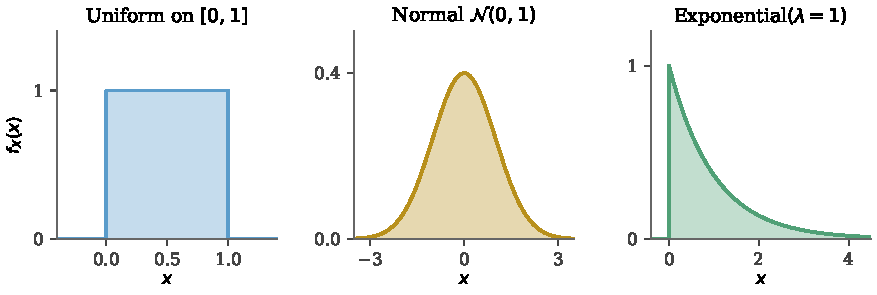
\includegraphics[width=\linewidth]{figures/ch01/pdf-curves.pdf}
\caption[Three PDFs side by side: Uniform, Normal, Exponential.]{Three densities at standard parameter values. The Uniform on $[0,1]$ is constant on its support; the Normal $\mathcal{N}(0,1)$ is the bell curve centred at zero; the Exponential$(1)$ decays from a finite peak at zero. Areas under all three curves are $1$.}
\label{fig:pdf-curves}
\end{figure}

% --- §1.2.4 The CDF: unifying object ----------------------------------------

\subsection*{The cumulative distribution function: a unifying object}

The PMF and PDF are different kinds of objects, applicable to different kinds of random variables. Is there a single function that handles both? Yes. It is the cumulative distribution function.

\begin{definition}{Cumulative distribution function (CDF)}{cdf}
The \emph{cumulative distribution function} of a random variable $X$ is the function $F_X : \R \to [0, 1]$ defined by
\[
F_X(x) \;=\; \Prob(X \le x).
\]
The CDF is non-decreasing, satisfies $\lim_{x \to -\infty} F_X(x) = 0$ and $\lim_{x \to \infty} F_X(x) = 1$, and is right-continuous.
\end{definition}

The CDF is defined for \emph{every} random variable, discrete or continuous. The PMF and PDF are recoverable from it.

\begin{proposition}{Recovering the PMF / PDF from the CDF}{pmf-pdf-from-cdf}
\textit{Let $X$ have CDF $F_X$.}
\begin{itemize}
\item \textit{If $X$ is discrete, the PMF is the jump heights of the CDF: $p_X(x) = F_X(x) - F_X(x^-)$, where $F_X(x^-) = \lim_{y \uparrow x} F_X(y)$.}
\item \textit{If $X$ is continuous and $F_X$ is differentiable at $x$, the PDF is the derivative: $f_X(x) = F_X'(x)$.}
\end{itemize}
\end{proposition}

\begin{proof}[Sketch]
For discrete $X$, the event $\{X \le x\}$ minus the event $\{X < x\}$ is exactly $\{X = x\}$, so the right-side jump of $F_X$ at $x$ has height $\Prob(X = x) = p_X(x)$. For continuous $X$, the fundamental theorem of calculus gives $\frac{d}{dx} \int_{-\infty}^{x} f_X(t)\, dt = f_X(x)$.
\end{proof}

The CDFs of our running examples have three quite different shapes. \Cref{fig:cdf-trio} shows them side by side.

\begin{figure}[h]
\centering
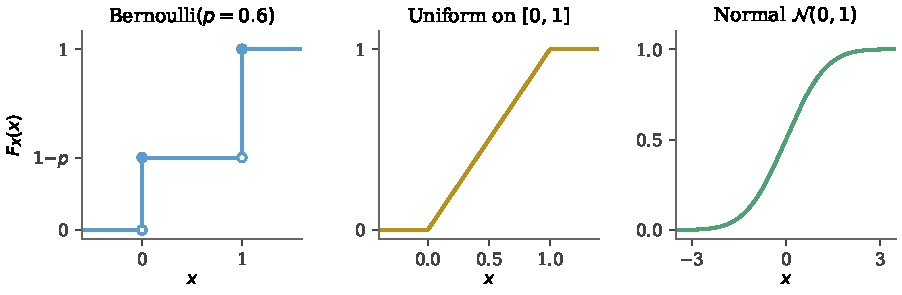
\includegraphics[width=\linewidth]{figures/ch01/cdf-trio.pdf}
\caption[Three CDFs: Bernoulli, Uniform, Normal.]{The CDF of a discrete random variable is a staircase (Bernoulli$(0.6)$, left); the CDF of a uniformly distributed random variable is a linear ramp (Uniform on $[0,1]$, middle); the CDF of a Normal is a smooth S-curve (centre, right). All three are non-decreasing and approach $1$ as $x \to \infty$.}
\label{fig:cdf-trio}
\end{figure}

% --- §1.2.5 Reference table -----------------------------------------------

\subsection*{A reference table of standard distributions}

The book leans on the same handful of standard distributions repeatedly. \Cref{tab:standard-distributions} gathers them in one place; later chapters point back to this table rather than re-defining each distribution.

\begin{table}[h]
\centering
\renewcommand{\arraystretch}{1.4}
\begin{fullwidth}
\footnotesize
\begin{tabular}{@{}llllll@{}}
\toprule
\textbf{Name} & \textbf{Type} & \textbf{Support} & \textbf{PMF / PDF} & \textbf{Mean} & \textbf{Variance} \\
\midrule
Bernoulli$(p)$ & discrete & $\{0, 1\}$ & $p_X(1) = p,\ p_X(0) = 1-p$ & $p$ & $p(1-p)$ \\
Binomial$(n, p)$ & discrete & $\{0, 1, \ldots, n\}$ & $\binom{n}{k} p^k (1-p)^{n-k}$ & $np$ & $np(1-p)$ \\
Geometric$(p)$ & discrete & $\{1, 2, 3, \ldots\}$ & $(1-p)^{k-1} p$ & $1/p$ & $(1-p)/p^2$ \\
Poisson$(\lambda)$ & discrete & $\{0, 1, 2, \ldots\}$ & $e^{-\lambda} \lambda^k / k!$ & $\lambda$ & $\lambda$ \\
\midrule
Uniform$(a, b)$ & continuous & $[a, b]$ & $1/(b-a)$ on $[a, b]$ & $(a+b)/2$ & $(b-a)^2 / 12$ \\
Exponential$(\lambda)$ & continuous & $[0, \infty)$ & $\lambda e^{-\lambda x}$ & $1/\lambda$ & $1/\lambda^2$ \\
Normal$(\mu, \sigma^2)$ & continuous & $\R$ & $\frac{1}{\sigma \sqrt{2\pi}} e^{-(x-\mu)^2 / (2\sigma^2)}$ & $\mu$ & $\sigma^2$ \\
\bottomrule
\end{tabular}
\end{fullwidth}
\caption{The standard distributions used throughout this book. Mean and variance are derived in \cref{ch:genfunc} via moment generating functions.}
\label{tab:standard-distributions}
\end{table}

% --- §1.2.6 Distribution sandbox ------------------------------------------

\subsection*{The distribution sandbox}

Reading a PDF or PMF formula on a page is one thing; watching a simulator throw thousands of samples and seeing the histogram resolve into the theoretical shape is another. \Cref{fig:sandbox-sample} shows a snapshot from the companion Colab notebook: $5{,}000$ samples from $\mathrm{Bin}(20, 0.3)$ on the left and from $\mathcal{N}(0, 1)$ on the right, each plotted against the theoretical PMF or PDF.\anchorDot{4}

\marginnote{%
\centering
\anchorDot{4}\,\sffamily\footnotesize\scshape Distribution sandbox\par
\smallskip
\colablink{Open notebook}{https://github.com/arzaansingh/mathemagics/tree/main/colab-notebooks/ch01-distribution-sandbox.ipynb}\par
\medskip
\itshape\footnotesize Generate samples, compare to theory, vary $N$.
}

\begin{figure}[h]
\centering
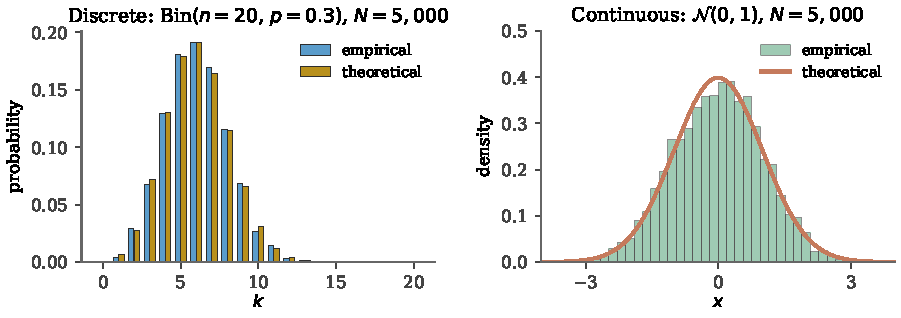
\includegraphics[width=\linewidth]{figures/ch01/sandbox-sample.pdf}
\caption[Sandbox sample: empirical histogram vs theoretical PMF / PDF.]{Empirical histogram (left bars / shaded) overlaid with the theoretical PMF / PDF (right bars / smooth curve) for two distributions, $N = 5{,}000$ samples each. With this many samples the two are visually indistinguishable; with $N = 50$ they would not be.}
\label{fig:sandbox-sample}
\end{figure}

The companion notebook \texttt{ch01-distribution-sandbox.ipynb} runs the same simulation interactively and lets the reader vary $N$, the sample size, to watch the empirical bars converge to the theoretical curves. The convergence is one form of the \emph{law of large numbers}, which we prove in \cref{ch:convergence}.

% --- §1.2.7 Brief warm-ups -----------------------------------------------

\subsection*{Brief warm-ups}

\hint{\anchorDot{5}\,Count the eight equally-likely strings $HHH, HHT, \ldots, TTT$, then group by number of heads.}
\begin{warmup}[\coffee{1}]
Let $X \sim \mathrm{Bin}(3, \tfrac{1}{2})$.\anchorDot{5} List $p_X(k)$ for $k = 0, 1, 2, 3$ and verify they sum to $1$.
\end{warmup}
\begin{warmupSolution}
$p_X(0) = \tfrac{1}{8}$, $p_X(1) = \tfrac{3}{8}$, $p_X(2) = \tfrac{3}{8}$, $p_X(3) = \tfrac{1}{8}$. The four values sum to $1$. (This is also the answer to Warm-up 1 of \cref{sec:rvs-samplespace}, viewed through the PMF.)
\end{warmupSolution}

\hint{\anchorDot{1}\,Integrate the constant density over the interval; equivalently, take the length of the subinterval.}
\begin{warmup}[\coffee{1}]
For $X \sim \mathrm{Uniform}(0, 1)$,\anchorDot{1} compute $\Prob(0.2 \le X \le 0.7)$ and sketch the CDF $F_X$ on the interval $[0, 1]$.
\end{warmup}
\begin{warmupSolution}
$\Prob(0.2 \le X \le 0.7) = 0.5$. The CDF is a linear ramp on $[0, 1]$: $F_X(x) = x$ for $x \in [0, 1]$, with $F_X(x) = 0$ for $x < 0$ and $F_X(x) = 1$ for $x > 1$.
\end{warmupSolution}

\hint{\anchorDot{2}\,A PDF must integrate to $1$ over its full support.}
\begin{warmup}[\coffee{2}]
Suppose $X$ is continuous with PDF $f_X(x) = c x$ for $x \in [0, 2]$, and $f_X(x) = 0$ otherwise.\anchorDot{2} Find the constant $c$.
\end{warmup}
\begin{warmupSolution}
$\int_0^2 c x \, dx = 2c = 1$, so $c = \tfrac{1}{2}$.
\end{warmupSolution}

\hint{\anchorDot{3}\,Integrate $\lambda e^{-\lambda t}$ from $0$ to $x$ to get $F_X(x)$.}
\begin{warmup}[\coffee{2}]
For $X \sim \mathrm{Exp}(\lambda)$,\anchorDot{3} derive the CDF $F_X(x)$ from the PDF $f_X(x) = \lambda e^{-\lambda x}$ on $[0, \infty)$.
\end{warmup}
\begin{warmupSolution}
For $x \ge 0$, $F_X(x) = \int_0^x \lambda e^{-\lambda t} \, dt = 1 - e^{-\lambda x}$. For $x < 0$, $F_X(x) = 0$.
\end{warmupSolution}

\bigskip

% --- §1.2 ENDS HERE; §1.3 onward still placeholder ---

\section{Expectation and variance}
\PLACEHOLDER{§1.3: definition and intuition; linearity of expectation; variance and standard deviation; worked examples on the running distributions.}

\section{Independence and joint distributions}
\PLACEHOLDER{§1.4: two random variables at once; joint and marginal distributions; independence and its consequences; second Colab simulation (joint plots for independent RVs).}

\section{Brief warm-ups and chapter recap}
\PLACEHOLDER{§1.5: 3--5 cross-section warm-ups; chapter recap box.}

\chapterRecap{%
\begin{itemize}
  \item \PLACEHOLDER{Punchline 1.}
  \item \PLACEHOLDER{Punchline 2.}
  \item \PLACEHOLDER{Punchline 3.}
\end{itemize}%
}

\section*{Exercises}
\PLACEHOLDER{8--15 longer exercises; solutions in Appendix A.}
